\chapter{Running a LLVM Pass}
\label{chap:chapter6}

\section{Installing Clang}
\label{InstallClang}
First install \href{https://clang.llvm.org/}{Clang} using 
\textbf{'sudo apt-get install'} command. Also, make sure that its 
version is compatible with the version of LLVM to be used.

\textbf{Note} - Install clang-8 (using \textbf{'sudo apt-get install 
clang-8'}) for working with LLVM-8.0.1, which is the current version.


\section{Building LLVM from source}
\label{BuildLLVM}

First ensure that \textbf{cmake} is installed on the system. For any 
further help on building LLVM from source, see 
\href{https://llvm.org/docs/CMake.html}{the LLVM documentation page}.

\begin{itemize}
    \item First download the LLVM source code from 
    \href{http://releases.llvm.org/download.html}{LLVM download page} 
    or use \href{https://github.com/llvm/llvm-project/releases/download/llvmorg-8.0.1/llvm-8.0.1.src.tar.xz}{this link}
    to download source code for LLVM-8.0.1. 
    \item Extract the LLVM source from the tar-package, at some 
    preferable location. The root folder of the source will now be 
    referred to as \textbf{LLVMsrc}.
    \item Create a new directory, which would be used for building 
    the LLVM source. This directory would be referred to as 
    \textbf{LLVMbuild}.
    \item Run \textbf{'cmake LLVMsrc'} from the \textit{LLVMbuild} 
    directory. CMake will detect the development environment, perform 
    a series of tests, and generate the files required for building 
    LLVM. 
    \item Run \textbf{'cmake -{}-build .'} from the \textit{LLVMbuild}
    directory to build the source.

    \textbf{Note} - This step might take hours to finish. Also, 
    building has very high memory requirements so it might also fail. 
    In this case repeat the last step and \textit{cmake} would detect 
    the packages it has already built in the previous run, and start 
    from where it was interrupted.
\end{itemize}
        
\section{Getting LLVM IR using Clang}
\begin{figure}[!h]
    \centering
    {
    \setlength{\fboxsep}{8pt}    
    \fbox{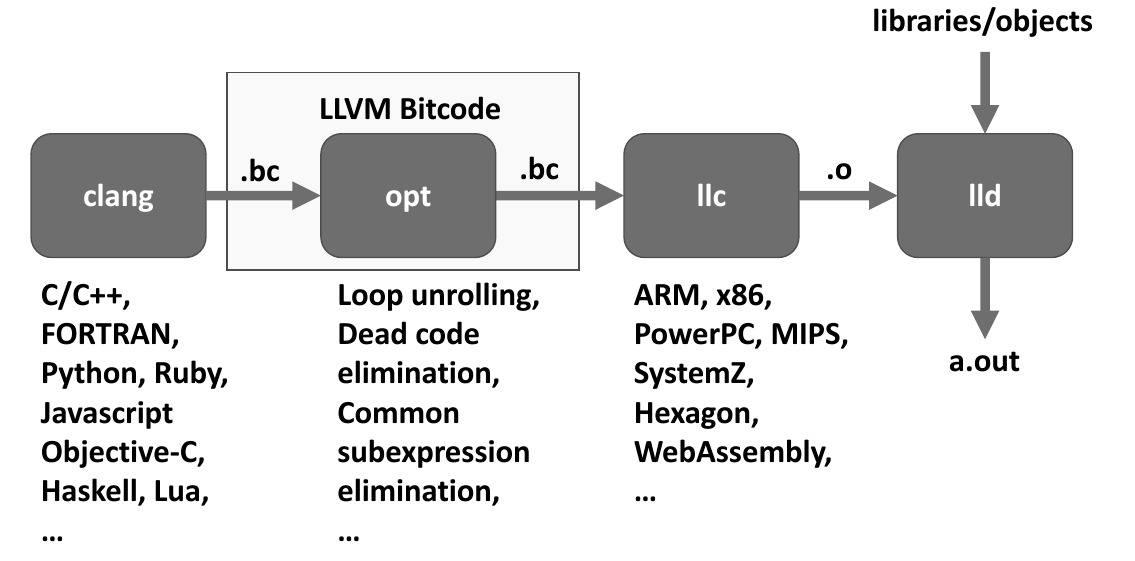
\includegraphics[scale=0.3]{LLVMcompiler.jpg}}
    }
    \caption{Various stages of compilation using Clang}
    \label{fig:LLVMcompiler}
\end{figure}

To compile a C file named \textit{hello.c} and get its 
\textit{LLVM intermediate representation} (IR) use the following 
commands. We can also give the name of the output file in both of the 
below commands using \textbf{\textit{'-o'}} flag.
\begin{itemize}
    \item \textbf{clang -emit-llvm -c hello.c} - This will give LLVM 
    bitcode in binary format file \textit{hello.bc}.
    \item \textbf{clang -emit-llvm -S hello.c} - This will give LLVM 
    code in text format file \textit{hello.ll}.
\end{itemize}
\textbf{Note} - Sometimes we may also need to specify the version 
along with \textbf{clang} (eg. clang-8), while running commands.
\\
We can also interconvert *.bc and *.ll file.
\begin{itemize}
    \item \textbf{LLVMbuild/bin/llvm-as hello.ll} - To convert 
    \textit{hello.ll} to \textit{hello.bc}
    \item \textbf{LLVMbuild/bin/llvm-dis hello.bc} - To convert \textit{hello.bc} to \textit{hello.ll}
\end{itemize}
We can also directly run *.bc or *.ll files as 
\textbf{'LLVMbuild/bin/lli hello.bc'} or 
\textbf{'LLVMbuild/bin/lli hello.ll'} respectively.

\section{Writing a pass}
In this section we will create a simple pass named \textit{HelloPass}.
\begin{itemize}
    \item Create directory \textit{'LLVMsrc/lib/Transforms/HelloPass'}. This directory will contain the files related to our pass.
    \item Create a new file named \textit{helloPass.cpp} inside \textit{HelloPass} directory. This file will contain the code for our pass.
        \begin{lstlisting}
#include "llvm/ADT/Statistic.h"
#include "llvm/IR/Function.h"
#include "llvm/Pass.h"
#include "llvm/Support/raw_ostream.h"
using namespace llvm;

namespace {
  struct helloPass : public FunctionPass {
    static char ID;
    helloPass() : FunctionPass(ID) {}

    bool runOnFunction(Function &F) override {
      errs() << "Function Name: ";
      errs().write_escaped(F.getName()) << '\n';
      errs() << "===================================================\n";
      for(auto bb = F.begin(); bb != F.end(); bb++){
        errs() << "\tBasicBlock Name = " << bb->getName() << "\n";
        errs() << "\tBasicBlock Size = " << bb->size() << "\n";
        for(auto i = bb->begin(); i != bb->end(); i++){
          errs() << "\t" << "Instruction: " << *i << "\n";
          errs() << "\t" << "OpCode: " << i->getOpcode() << "\n";
          errs() << "\t" << "OpCodeName: " << i->getOpcodeName() << "\n";
          errs() << "\t" << "IsBinaryOp: " << i->isBinaryOp() << "\n";
          errs() << "\t" << "IsCommutative: " << i->isCommutative() << "\n";
          errs() << "\t" << "IsAssociative: " << i->isAssociative() << "\n";
        }
        errs() << "\n\n";
      } 
      return false;
    }
  };
}
char itrinstBB::ID = 0;
static RegisterPass<helloPass> X("hello", 
                                 "Iterates instructions in a function");
        \end{lstlisting}
        The above code contains a function pass - which means the 
        pass is run on every function defined in a file. Using 
        iterators it traverses each basic block of the function, and 
        for each basic block, it traverses each instruction and 
        prints the details of the instruction - like its opcode, 
        whether it is commutative and associative etc.\\
        \textbf{Important} - Notice the first argument \textbf{hello} 
        which is passed in the last line while registering the pass. 
        This argument will be passed as a flag to the 
        \textit{HelloPass} pass when we want to run the function-pass 
        defined inside \textit{helloPass} structure (the template 
        arguments in the last line).
    \item Create a file named \textit{CMakeLists.txt} in the same 
    HelloPass dirctory. This file will be used by \textbf{make} when 
    building the pass.
        \begin{lstlisting}
add_llvm_library( LLVMhelloPass MODULE
  helloPass.cpp
  PLUGIN_TOOL
  opt
)
        \end{lstlisting}
        \textit{LLVMhelloPass} in the first line specifies the 
        filename (with *.so extension) inside \textit{LLVMbuild/lib/}
        directory, which will contain our pass when built. 
        \textit{helloPass.cpp} in the second line specifies the file 
        which contains the source code for our pass.
    \item Add the following line to the file 
    \textit{'LLVMsrc/lib/Transforms/CMakeLists.txt}
        \begin{lstlisting}
add_subdirectory(HelloPass)
        \end{lstlisting}
        This is the name of folder which contains our pass and will be used by \textbf{make} while building.

\end{itemize}

\textit{Note} - More detailed tutorial on writing a pass can be found 
\href{http://llvm.org/docs/WritingAnLLVMPass.html#quick-start-writing-hello-world}{here}.

\section{Running a pass}
\begin{itemize}
    \item Firstly rebuild the LLVM source so that it includes the 
    pass we have added. For this change current directory to \textit
    {LLVMbuild} and run \textbf{\textit{make}}.
    \item Now run the pass on an LLVM bitcode file 
    \textit{helloWorld.ll} or \textit{helloWorld.bc} as \\
        \textbf{'./bin/opt -load ./lib/LLVMhelloPass.so -hello hello.ll -o helloN.bc'}\\
        Notice that \textit{LLVMhelloPass} is the name that we 
        specified in the \textit{CMakeLists.txt} file of our pass 
        folder. Also, \textit{-hello} flag is the name by which we 
        registered our pass in the end of the file \textit
          {helloPass.cpp}

\end{itemize}